\section{System Architecture Overview}
\label{sec:system-architecture-overview}

Stockrium follows a client--server architecture supported by independent background and offline data-acquisition pipelines. The React Native mobile application is the primary interface for individual investors, while an internal experimentation and backtesting web interface allows authorized evaluators to run controlled analysis and historical experiments. Both clients communicate with a FastAPI backend that centralizes authentication, business logic, data access, agentic AI and conversational workflows, and standardized API responses.

Supabase PostgreSQL stores the application's durable business, market, financial, news, and conversational data, while Redis maintains temporary authentication and verification state. Separate workers collect and prepare information from external sources such as SSI and online news providers. This separation keeps provider credentials and processing logic outside the clients and allows most user requests to read normalized data that have already been prepared.

\subsection{Architectural Requirements}
\label{subsec:architectural-requirements}

The architecture must support mobile market exploration, configurable agentic AI analysis, conversational queries, and controlled backtesting without coupling these responsibilities to the user interface. It must integrate heterogeneous financial evidence, protect user-specific and restricted experimentation operations, preserve conversation state, and update market and news data without blocking normal requests. Maintainability is supported by separating presentation, domain services, agentic AI and conversational workflows, and data access. Most importantly, the architecture reflects the application's decision-support scope: no component connects to a brokerage account, transfers funds, or executes securities transactions.

Several quality attributes influence this organization. Security requires provider keys and privileged data access to remain on the server side. Responsiveness requires ordinary mobile requests to read prepared records instead of waiting for crawlers or large imports. Maintainability requires the API, analytical workflows, and acquisition jobs to evolve independently, while traceability is supported by structured results and persistent records for conversations and historical experiments. The architecture therefore prioritizes clear responsibility boundaries, traceable processing, and repeatable evaluation rather than the low-latency execution required by a trading platform.

\subsection{Logical Architecture}
\label{subsec:logical-architecture}

The logical architecture is organized into presentation, API and application services, AI and evaluation, data integration, and persistence. Background workers connect external providers to the data layer independently of user requests. Figure~\ref{fig:stockrium-overall-architecture} summarizes the principal components and their relationships.

\begin{figure}[H]
    \centering
    \IfFileExists{figures/chapter4/stockrium_client_server_architecture.png}{%
        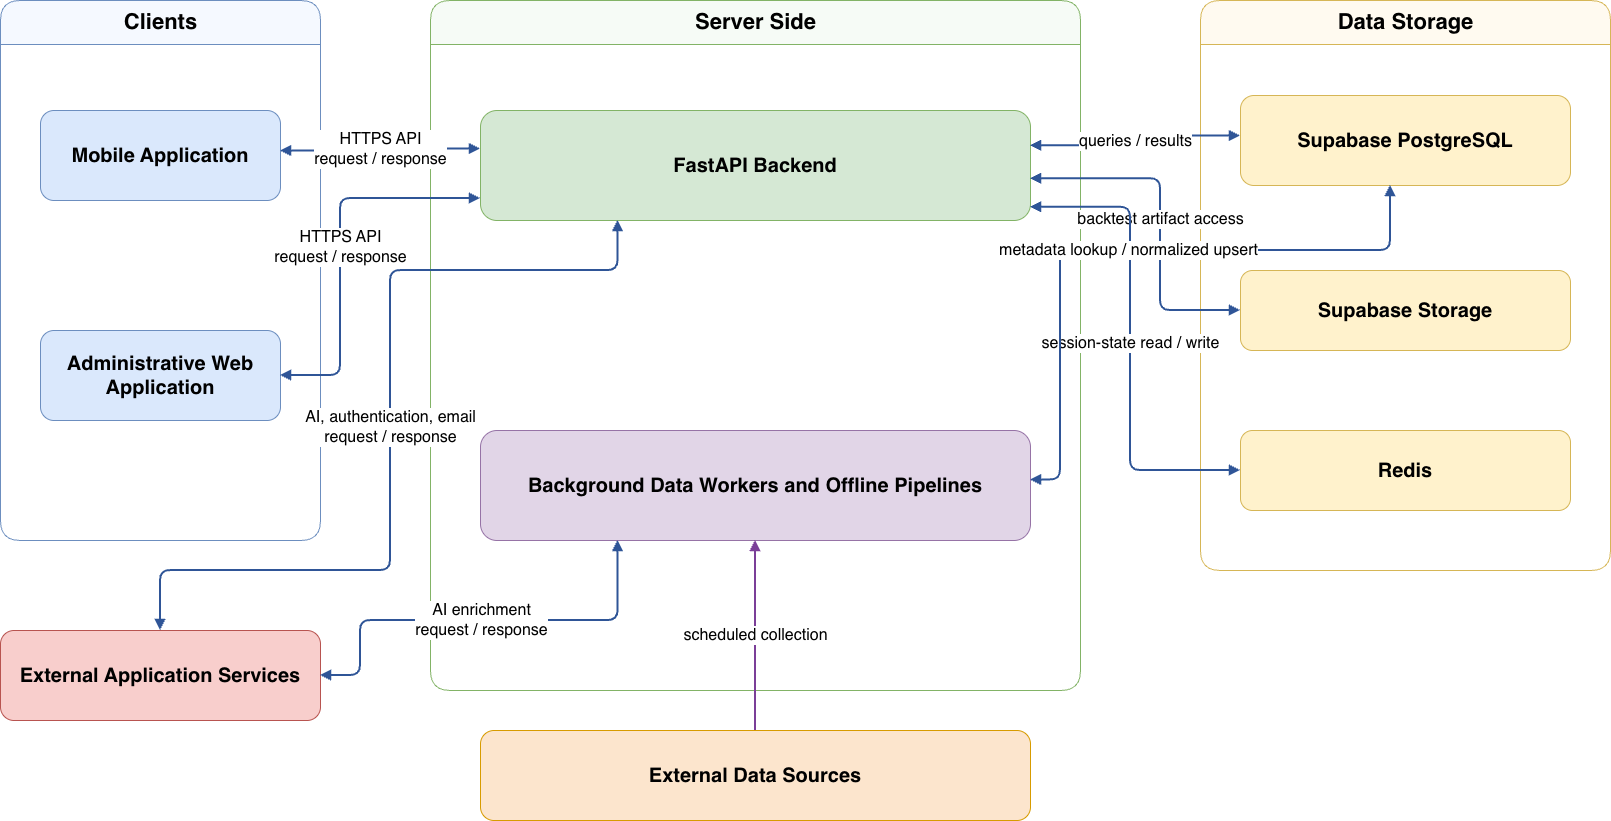
\includegraphics[width=\textwidth,height=0.78\textheight,keepaspectratio]{figures/chapter4/stockrium_client_server_architecture.png}%
    }{%
        \fbox{\parbox[c][5.5cm][c]{0.92\textwidth}{\centering
        Export the Draw.io diagram as\\
        \texttt{figures/chapter4/stockrium\_client\_server\_architecture.png}}}%
    }
    \caption{Overall logical architecture of Stockrium}
    \label{fig:stockrium-overall-architecture}
\end{figure}

On the client side, the mobile application and experimentation web interface serve different actors while sharing the same server boundary. The mobile application supports everyday investor activities, including authentication, market discovery, stock details, charts, news, the watchlist, investment-horizon management, AI-assisted analysis, and conversational follow-up. It retains only interface state, user preferences, and securely stored authentication tokens; authoritative financial and user data remain on the server. The experimentation interface is restricted to authorized evaluators. It supports AI-assisted analysis for an individual stock, VN30, or VN100 and backtesting for an individual stock or VN30, together with progress monitoring, result inspection, and export. Backtesting evaluates Stockrium's analytical pipeline and supported configurations; it is not a general-purpose strategy builder or a publicly deployed web equivalent of the mobile product.

On the server side, FastAPI acts as the single entry point for Stockrium application requests from both clients. It validates request schemas, authenticates the current session, checks elevated-role authorization where required, invokes the relevant application service, and returns the standardized Stockrium response structure. Domain services organize operations for accounts, market data, company profiles, financial statements, articles, watchlists, search history, and investment horizons. This route--service separation prevents the clients from depending on database-specific queries and permits the same business operations to be reused by analytical workflow components, chatbot tools, or backtesting services.

The server also owns the computation-intensive and security-sensitive capabilities. The stock-analysis workflow coordinates technical, fundamental, and news evidence before producing a structured recommendation. The conversational workflow maintains multi-turn state and selects suitable financial tools, while the backtesting subsystem applies the analytical logic to historical data under supported backtest inputs. These components may call external language-model services, but API keys, prompts, validation rules, and post-processing remain within the server-side environment. Their internal designs are described separately later in this chapter.

The storage side is divided according to data lifetime and format. Supabase PostgreSQL is the authoritative relational store for accounts, personalization, stocks, prices, market indices, company records, financial statements, articles, classifications, chat-session metadata, and LangGraph checkpoints. Supabase Storage holds backtest artifacts that are more suitable as files than relational rows. Redis stores revocable or short-lived authentication state, including access and refresh token registrations, one-time passwords, attempt counters, and password-reset sessions. Interactive client operations retrieve and update these stores through the FastAPI backend, while authorized acquisition workers access the required data stores independently of client requests.

Background workers form a second server-side execution path that is independent of interactive API requests. The market-price worker receives SSI data, prepares intraday and daily records, and performs post-session normalization. The article worker discovers and extracts financial news, checks duplicates, generates summaries and sentiment labels, links articles to stocks or categories, and persists the processed results. Company and fundamental utilities collect profile and financial information through Selenium and downloadable files before transforming it with pandas. These jobs can read database metadata or existing records before upserting normalized results into PostgreSQL.

External application services support both synchronous and background operations. OpenAI models are used by the analytical workflows and selected enrichment jobs, while Resend delivers account-verification email. These services are accessed by the backend or workers so that credentials and output validation remain in the server-side environment. Google Sign-In follows a different boundary: the mobile application initiates authentication with Google Identity, receives an identity token, and sends it to the backend for verification and issuance of Stockrium access and refresh tokens. None of these request--response integrations is an authoritative source of Stockrium's business or market records.

\subsection{End-to-End Request Flows}
\label{subsec:end-to-end-request-flows}

For an ordinary data-retrieval request, a client sends a Hypertext Transfer Protocol (HTTP) request to FastAPI and includes a Stockrium authentication token where required; deployed mobile requests use Hypertext Transfer Protocol Secure (HTTPS). The route validates the input and resolves the current user before invoking a domain service. The service reads the corresponding prepared records from PostgreSQL, applies any required transformation, and returns them through the standard response envelope. The client then maps the response into cards, lists, charts, or detail views. User actions such as updating the watchlist, search history, or investment horizon follow the same path but write the authorized change before returning the updated state.

An AI-analysis request follows the same client--server boundary but invokes a server-side graph after the relevant market, fundamental, and news evidence has been retrieved. Only the selected analytical components participate, and their outputs are synthesized and validated before the result is returned to the client. A conversational request additionally loads and updates its LangGraph checkpoint, whereas a controlled backtest repeatedly applies analytical logic to historical records and may expose or store an experiment artifact. Although these operations differ in duration and state, none bypasses backend authentication or grants a client direct access to the database or model provider.

Data acquisition follows a path independent of interactive requests. At scheduled times, during market hours, or through a controlled offline preparation run, a worker or utility reads from its external provider, normalizes the received representation, checks required database context, and upserts the prepared data into PostgreSQL. The FastAPI service later reads the resulting records in response to client requests. Separating this path from the web-server lifecycle prevents a market stream, browser crawler, article-processing batch, or large import from delaying ordinary API traffic and avoids duplicating scheduled jobs when the API process restarts or scales.

Overall, Stockrium combines thin client applications, a validated FastAPI boundary, modular domain and AI services, independent acquisition pipelines, and storage selected according to data lifetime. The following sections describe each of these areas in greater detail.
